% THIS IS AN EXAMPLE DOCUMENT FOR VLDB 2012
% based on ACM SIGPROC-SP.TEX VERSION 2.7
% Modified by  Gerald Weber <gerald@cs.auckland.ac.nz>
% Removed the requirement to include *bbl file in here. (AhmetSacan, Sep2012)
% Fixed the equation on page 3 to prevent line overflow. (AhmetSacan, Sep2012)

\documentclass{vldb}
\usepackage{graphicx}
\usepackage{color}
\usepackage{balance}  % for  \balance command ON LAST PAGE  (only there!)
\usepackage{times}
\usepackage{url}
\usepackage{algorithm}
\usepackage[noend]{algorithmic}
\usepackage{subfigure}
\usepackage{xspace}
\usepackage[noend]{algorithmic}
\usepackage{enumerate}
\usepackage{multirow}
\usepackage{epstopdf}
\usepackage{cleveref}
\newcommand{\squishlist}{
   \begin{list}{$\bullet$}
    {
      \setlength{\itemsep}{0pt}
      \setlength{\parsep}{3pt}
      \setlength{\topsep}{3pt}
      \setlength{\partopsep}{0pt}
      \setlength{\leftmargin}{1.5em}
      \setlength{\labelwidth}{1em}
      \setlength{\labelsep}{0.5em} } }

\newcommand{\squishend}{
    \end{list}  }

\newcommand{\argmax}{\operatornamewithlimits{arg\ max}}

\newcommand{\eat}[1]{}
\newcommand{\todo}[1]{\textcolor{red}{{TODO: #1}}}
\newcommand{\add}[1]{\textcolor{red}{{ADD: #1}}}
\newcommand{\note}[1]{\textcolor{blue}{{#1}}}

\newtheorem{definition}{Definition}
\newtheorem{example}{Example}
\newtheorem{theorem}{Theorem}
\newtheorem{lemma}{Lemma}
\newtheorem{problem}{Problem}
\newtheorem{reduction}{Reduction}
\newcommand{\domain}{\mathcal{D}}
\newcommand{\attributes}{\mathcal{A}_D}
\newcommand{\hierarchy}{\mathcal{H}_D}
\newcommand{\attrhierarchy}{\mathcal{H}_A}
\newcommand{\workers}{\mathcal{W}}
\newcommand{\uentities}{\mathcal{E}}
\newcommand{\queryvector}{{\bf Q_S}}



\begin{document}

% ****************** TITLE ****************************************

\title{CrowdGather: Budgeted Entity Extraction over Structured Data Domains}

\numberofauthors{3} 

\author{
	\alignauthor Theodoros Rekatsinas\\
            \affaddr{University of Maryland, College Park} %, College Park MD 20742}
                \email{thodrek@cs.umd.edu}
            \alignauthor Amol Deshpande\\
            \affaddr{University of Maryland, College Park} %, College Park MD 20742}
                \email{amol@cs.umd.edu}
            \alignauthor Aditya Parameswaran \\
            \affaddr{University of Illinois, Urbana-Champaign University} %, Durham NC 27708}
                \email{adityagp@illinois.edu}
}

\maketitle

\begin{abstract}
Crowd entity extraction has become a popular means of acquiring data for many applications, including recommendation systems, listing aggregation and knowledge base compilation.  Most of the current solutions focus on entity extraction for specific queries and do not consider entity extraction over broader entity domains. Due to the time and cost of human labor, considering each query in isolation may incur large costs when applied to broader domains, thus, limiting the applicability of current approaches.
 
In this paper, we explore the problem of {\em budgeted entity extraction} over {\em structured entity domains}. We consider domains that can be fully described by a collection of attributes, each characterized by a hierarchical structure. We develop new statistical tools that enable users to reason about the gain of issuing {\em further queries} in the presence of little information and show how to exploit the dependencies across different points of the data domain to obtain more accurate estimates. We also demonstrate how budgeted entity extraction over large domains can be cast as an adaptive optimization problem that seeks to maximize the number of extracted entities while minimizing the overall extraction cost. We evaluate our techniques with experiments on both synthetic and real-world data. 
\end{abstract}

\section{Introduction}
\label{sec:intro}
Combining human computation with traditional computation has been recently proven beneficial in extracting knowledge and acquiring data for many application domains, including recommendation systems~\cite{amsterdamer:2014}, knowledge base completion~\cite{kondredi:2014}, entity extraction and structured data collection~\cite{trushkowsky:2013, park:2014}. In fact, extracting information, and entities in particular, from the crowd has been shown to provide access to more fine grained information that may belong to the long tail of the web or even be completely unavailable on the web~\cite{franklin:2011, Parameswaran:2012, west:2014}.

A fundamental challenge in crowdsourced entity extraction is reasoning about the completeness of the extracted information. More precisely, given a task that seeks to enumerate entities from a specific domain by asking human workers, e.g., ``extract all restaurants in New York", it is not easy to judge if we have extracted all entities (in this case restaurants). This is because we are in an ``open world"~\cite{trushkowsky:2013} scenario. Extracting entities from the crowd can be done by issuing {\em queries} of the form ``Give me $k$ entities corresponding to a specific domain". In our restaurant example, such queries may correspond to crowdsourced task of the form ``give me 5 French restaurant in Manhattan, NY". Recent work has considered this problem for isolated queries~\cite{trushkowsky:2013} , i.e., queries that correspond to exactly the same question and are repeatedly evaluated against workers. In this line of work, the query predicates specify the data domain of interest. 

Often, however, crowd entity extraction techniques are used to acquire information from large data domains that cannot be described adequately by a single query with fixed predicates. Consider for example a scenario where crowd sourcing techniques are used to collect information about various types of events (e.g., music concerts or political rallies) over different countries. If we just asked workers to provide us with events without specifying the event type or location, we would get a limited number of {\em popular} events. Moreover, the characteristics of collected events would heavily depend on the demographics of the workers completing the task. For example, a US based worker is more likely to provide us with events occurring in the state she is located. 

However, if we want to maximize the number of extracted events we can intuitively issue multiple diversified queries, requesting the crowd to provide information for specific types of events potentially focusing on a specific location. Notice, that following this approach we are less likely to be affected by heavily popular events and the worker specific characteristics. However, deciding on the right queries in such domains entails several challenges. Next, we use a real-world scenario to illustrate these challenges.

\subsection{Challenges and Opportunities}
\label{sec:challenges}
We consider Eventbrite~\footnote{https://www.eventbrite.com}, an online event aggregator, that relies on crowdsourcing to compile a directory of events with detailed information about the location, type, date and category of each event. Typically, event aggregators are interested in collecting information about diverse events spanning from conferences and music festivals to political rallies for multiple locations across different location, i.e., countries or cities. In particular, Eventbrite collects information about events across different countries in the world. Each country is further split into cities and areas across the country. Moreover, events are organized according to their type and topic. We collected a dataset from Eventbrite spanning over 63 countries that are divided into 1,709 subareas (e.g., states) and 10,739 cities, containing events of 19 different types, such as rallies, tournaments, conferences, conventions, etc. and a time period of 31 days spanning over the months of October and November. It is easy to see that two of the three dimensions, i.e., location and time, describing the domain of collected events  are hierarchically structured. The overall domain can be fully specified if we consider the cross product across the possible values for location, event type and time. For each of the location, time, type dimensions we also consider a special {\em wildcard} value. Taking the cross-product across the possible values of these dimensions results in a total of 8,508,160 points containing 57,805 distinct events overall.

The first challenge stems from the fact that due to the sheer size of the data domain there are potentially many sparsely populated points, i.e., points  that contain only a limited number of items. Assuming a given budget for crowdsourced entity extraction, one needs to avoid such points when issuing crowdsourced entity enumeration queries in order to maximize the number of extracted entities under the specified budget. 

\begin{example}
We focus on the collected Eventbrite dataset and plot the number of items for each of the data items associated the event domain under consideration. Out of 8,508,160 points only 175,068 points are associated with events while the remaining points have zero events. \Cref{fig:eventbritepop} shows the number of events associated with these point. Notice that the y-axis is in log-scale. As shown the majority of populated points have less than 100 items. It is obvious that when trying to extract events from such a sparse domain one needs to optimize the crowdsourced queries if operating under a monetary budget.
\end{example}

\begin{figure}
	\begin{center}
	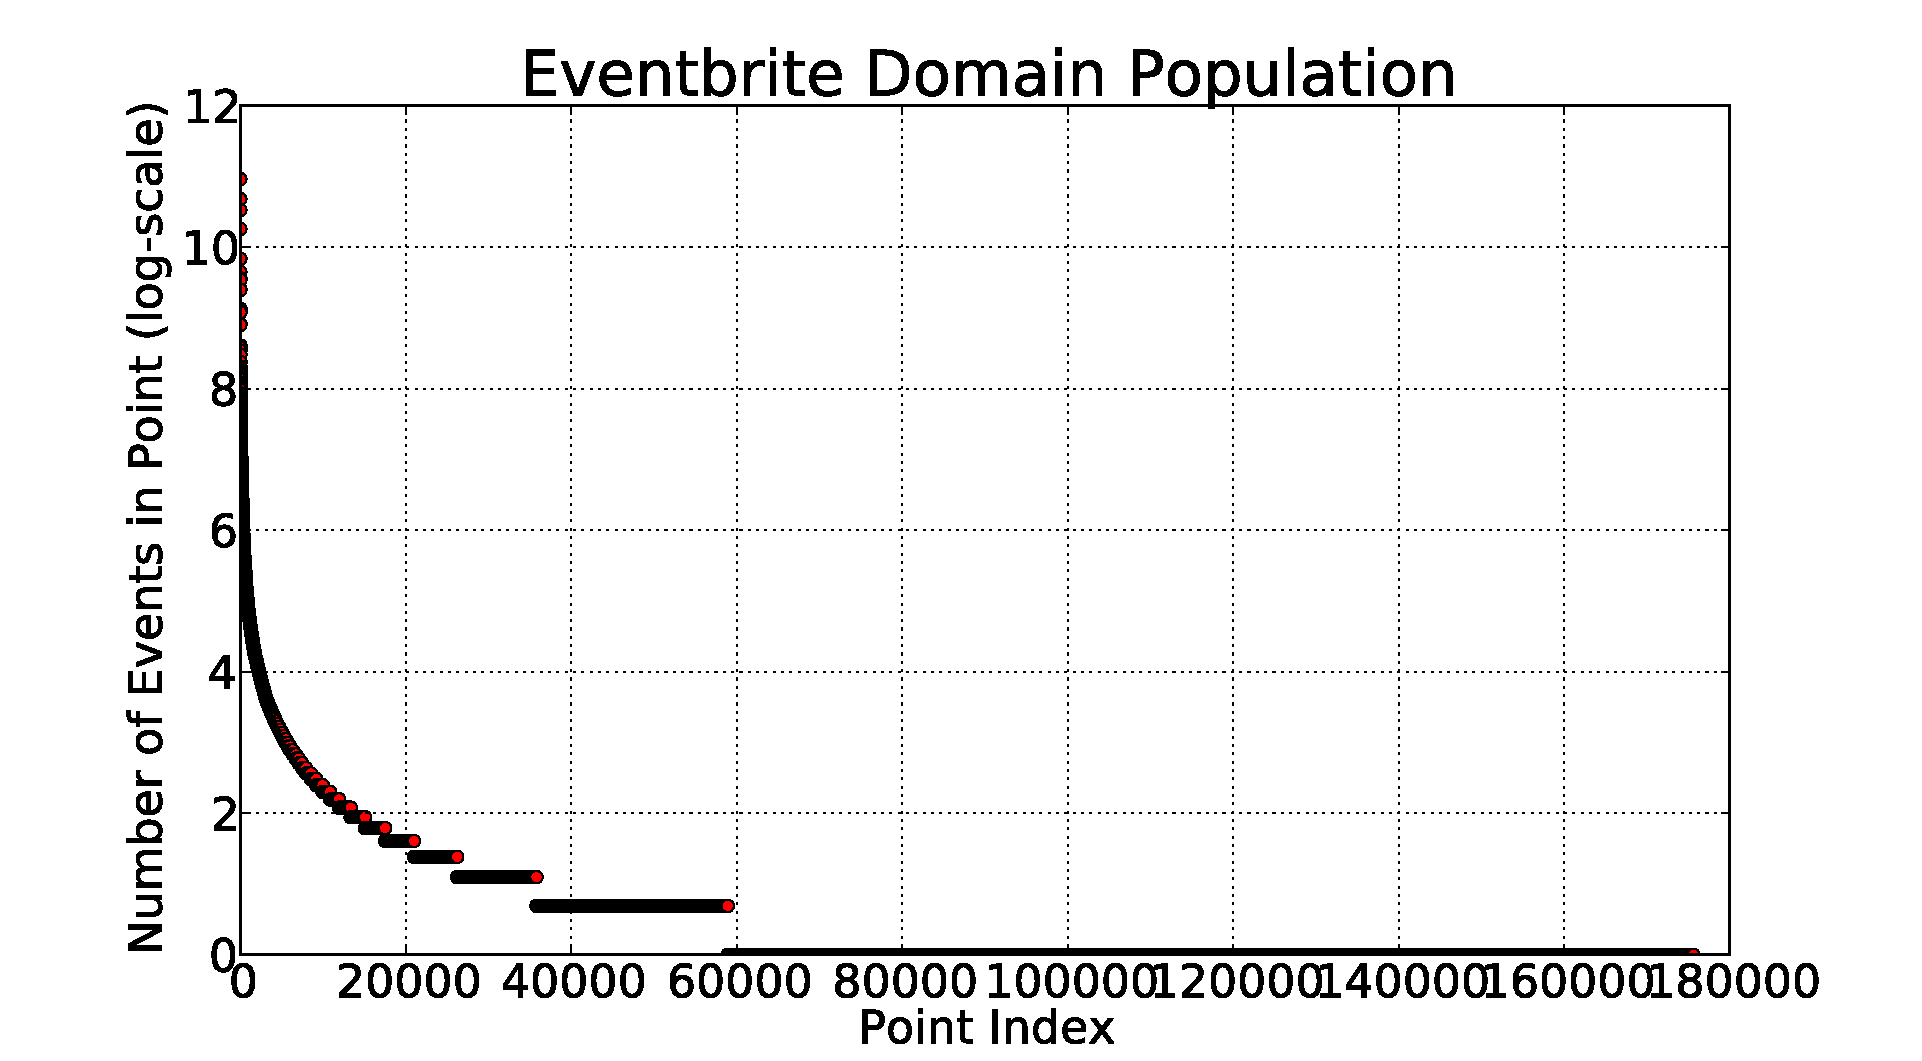
\includegraphics[trim=55 0 62 0,clip,scale=0.25]{figs/eventBritePopulationS.pdf}
	\caption{The attributes describing the events domain and the hierarchical structure of each attribute.}
	\label{fig:eventbritepop}
	\vspace{-20pt}
	\end{center}
\end{figure}

However, the hierarchical structure of the data domain presents us with an opportunity. In fact, we observe that the heavily populated domain points are not {\em leaf points}, i.e., points for which all the dimension values are specified but points for which one or more dimensions are assigned the wildcard value and thus can obtain any value. In fact, one can exploit this to maximize the number of extracted entities as we further discuss in \Cref{sec:prelims}.

The second challenge when consider large domains such as the Eventbrite domain, is the overlaps among different points of the domain. More precisely, when we ask the crowd to provide us with entities associated with a domain specific point (e.g., events in New York) these entities may be associated with other points in the domain (e.g., concerts in New York). Therefore we indirectly obtain information about the population of domain points for which no queries may have been issues. 
These dependencies across queries pose a significant challenge when estimating the number of new entities obtain by a query.

\begin{example}
We consider again the Eventbrite dataset and plot the pairwise overlaps of the ten most populous points in the domain. \Cref{fig:enventbriteover} shows the Jackard index for the corresponding point pairs. As shown the event populations corresponding to these points overlap significantly. It is easy to see that when issuing queries at a certain domain point, we not only obtain events corresponding to this point but to other points in the domain as well. 
\end{example}

\begin{figure}
	\begin{center}
	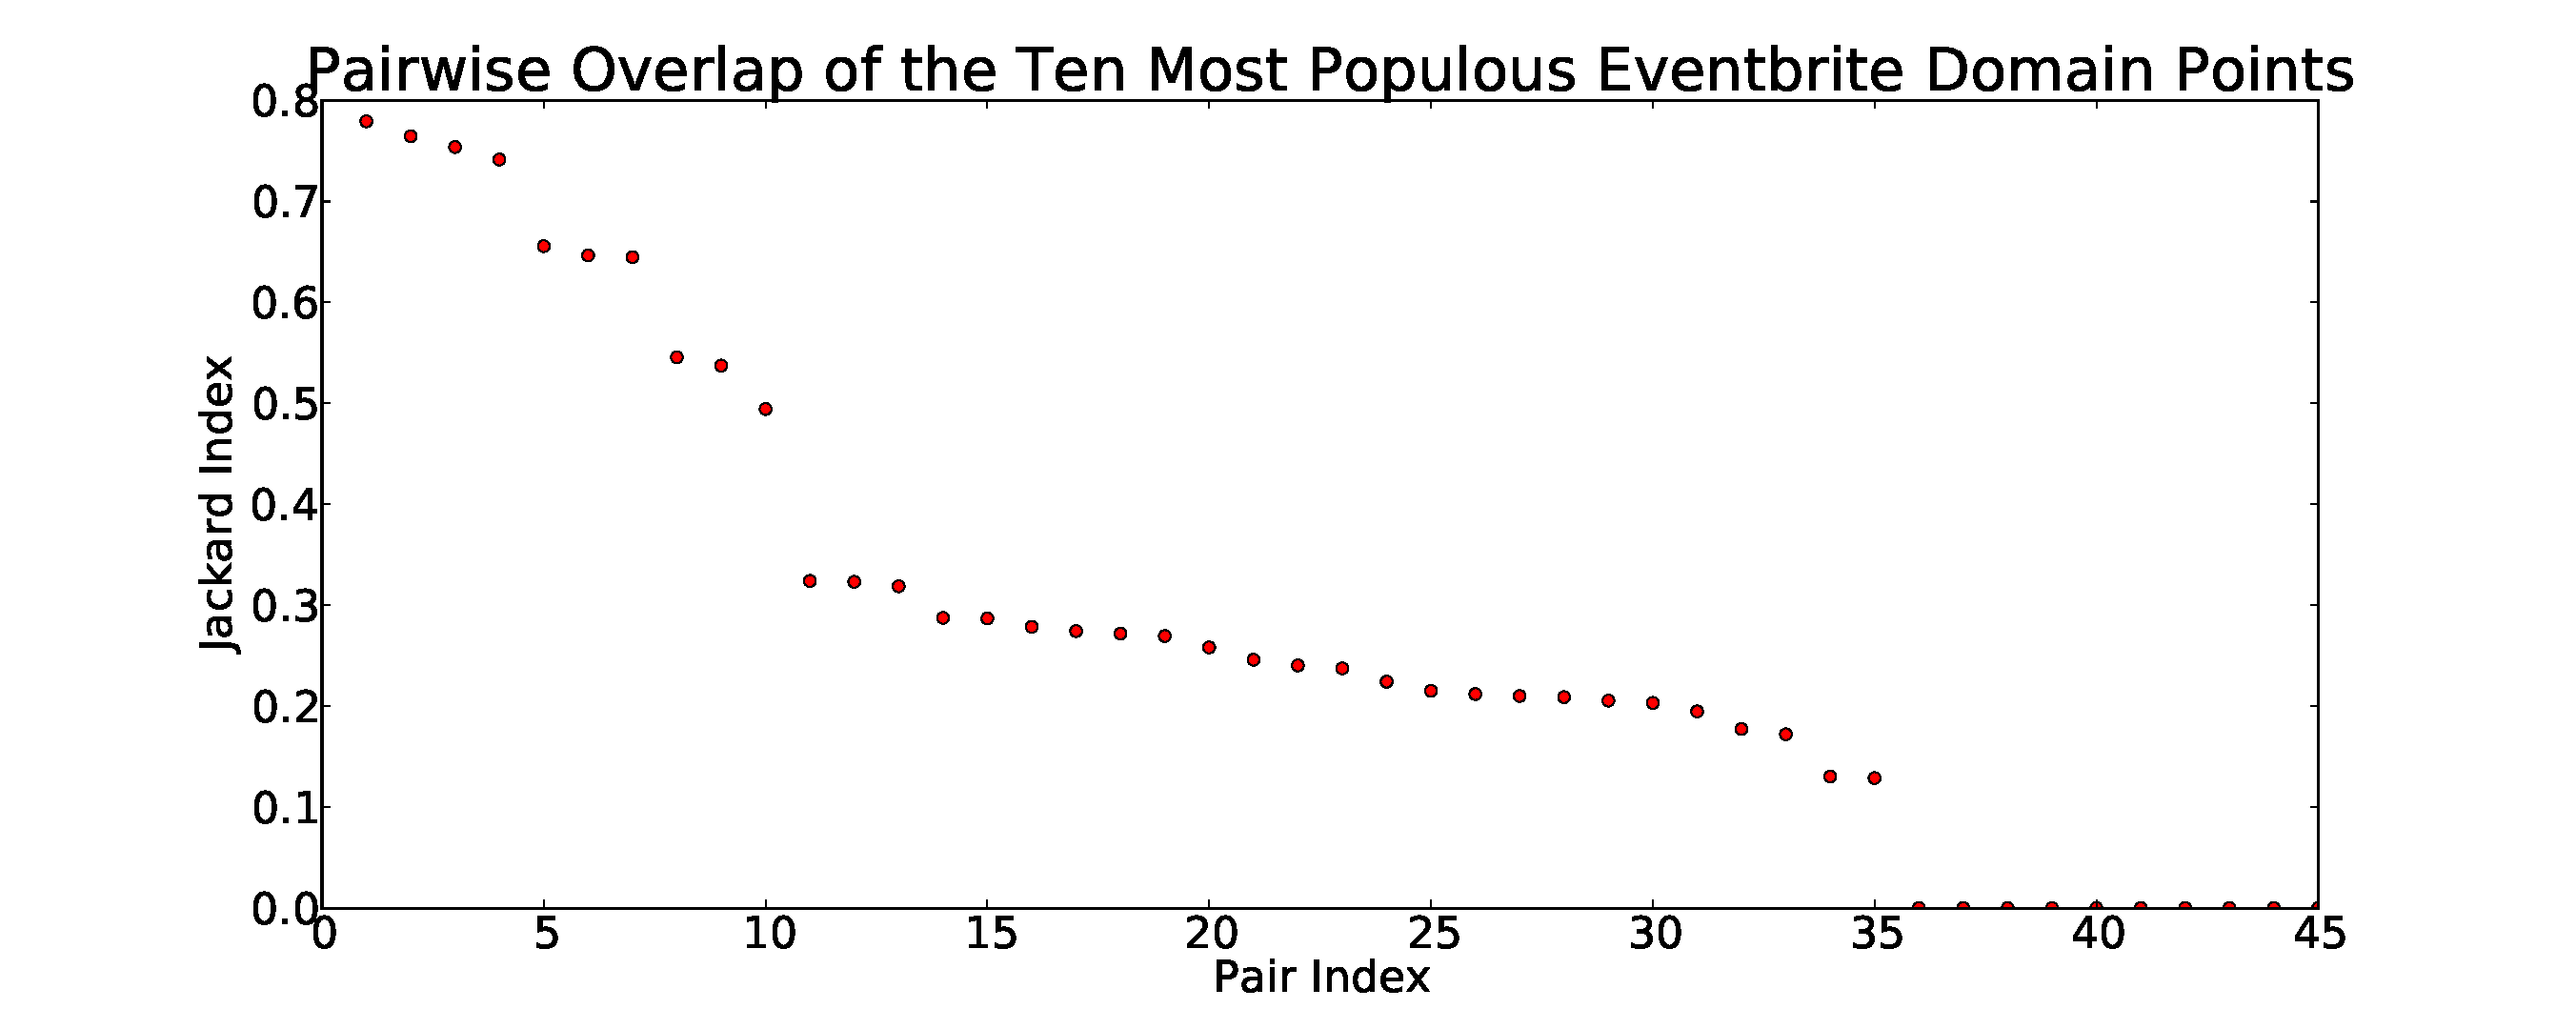
\includegraphics[trim=55 0 62 0,clip,scale=0.2]{figs/overlaps.pdf}
	\caption{Pairwise overlaps of the 10 most populous domain points in Eventbrite.}
	\label{fig:eventbriteover}
	\vspace{-20pt}
	\end{center}
\end{figure}

\subsection{Contributions}
\label{sec:contributions}
Motivated by these examples, we study the problem of {\em budgeted crowd entity extraction} over {\em structured domains}. More precisely, we focus on domains described by a collection of attributes, each following a known {\em hierarchical structure}, i.e., we assume that for each attribute the corresponding hierarchy is known.

We propose a novel algorithmic framework that exploits the structure of the domain to maximize the number of extracted entities under given budget constraints. In particular, we view the problem of entity extraction as a {\em multi-round adaptive optimization problem}. At  each round we exploit the information on extracted entities obtained by previous queries to adaptively select the crowd query that will maximize the {\em gain} and cost trade-off at each round. The gain of a query is defined as the number of new unique entities extracted by it. We extend on previous query interfaces that considered only questions of the type ``Give me $k$ more entities" and examine {\em generalized queries} that can also include an {\em exclude list}. In general such queries are of the type ``Give me $k$ more entities that are not $A$, $B$, etc". Building upon techniques from the species estimation and the multi-armed bandits literature, we introduce a new methodology for estimating the gain for such generalized queries and show how the hierarchical structure of the domain can be exploited to improve the accuracy of our gain estimates. Our main contributions are as follows:

\squishlist
\item We study the challenge of information flow across entity extraction queries for overlapping parts of the data domain.
\item We develop a new technique to estimate the gain of generalized entity extraction queries under the presence of dependent information. The proposed technique exploits the structure of the data domain to obtain accurate estimates. 
\item We introduce an adaptive optimization algorithm that takes as input the gain estimates for different types of queries and identifies querying policies that maximize the total number of retrieved entities under given budget constraints. 
\item Finally, we show that our techniques can effectively solve the problem of budgeted crowd entity extraction for large data domains on both real-world and synthetic data.
\squishend

\section{Preliminaries}
\label{sec:prelims}
In this section we first review different types of crowd query interfaces for entity extraction. The we focus on crowdsourced entity extraction using these interfaces and consider the problem of maximizing the number of extracted entities. In particular, we define the problem of {\em crowd entity extraction} over {\em structured domains} under budget constraints. Then, we formally introduce the challenge of dependencies across queries when extracting entities from structured domains, and finally, we present an overview of our proposed algorithmic framework.

\subsection{Entity Extraction Queries}
\label{sec:queries}
Let $\domain$ be a data domain described by a set of discrete attributes $\attributes = \{A_1, A_2, \dots, A_d\}$. Let $dom(A_i)$ denote the domain of each attribute $A_i  \in \attributes$.  We consider three different types of crowd queries for extracting entities from the crowd. The first type corresponds to {\em single entity queries} where workers are required to provide ``one more" entity that satisfies the collection of predicates over attributes in $\attributes$. Considering the Eventbrite example introduced in the previous section an example of a single entity query would be asking a worker to provide ``a concert in Manhattan, New York'". The second type of queries corresponds to {\em queries of  size k} where workers are asked to provide up to $k$ distinct entities. Finally, the last type corresponds to {\em exclude list queries}. Here,  workers are provided with $l$ entities that have already been extracted and are required to provide up to $k$ distinct entities under the constraint that none of them is included in the exclude list. It is easy to see that the last type of queries generalizes the previous two. Therefore, in the remainder of the paper, we will consider that all queries of the third type. To describe a query, we will use the notation $q(k,l)$ denoting a query of size $k$ accompanied with an exclude list of length $l$. 

In a typical crowdsourcing environment, tasks have different costs depending on their difficulty. Thus, crowdsourced queries of different difficulties should also exhibit different costs. Let $c(\dot)$ be a cost function for any query $q(k,l)$. This cost function should obey the following properties: (a) given an exclude list of fixed length $l$ then $c(q(k^{\prime},l)) \geq c(q(k,l)),  \forall k^{\prime} \geq k$, and (b) given a fixed query size $k$ then $c(q(k,l^{\prime})) \geq c(q(k,l)), \forall l^{\prime} \geq l$. These are fixed upfront by the interface designed based on the amount of work involved.

\subsection{Crowd Entity Extraction}
\label{sec:extraction}
We focus on structured domains where each attribute is hierarchically organized. For example, consider the Eventbrite domain introduced in \Cref{sec:challenges}. The data domain $\domain$ corresponds to all events and the attributes describing the entities in $\domain$ are $\attributes = \{$``Event Type", ``Location", ``Date"$\}$. \Cref{fig:eventsdomain} shows the hierarchical organization of each attribute.

\begin{figure}[h]
	\begin{center}
	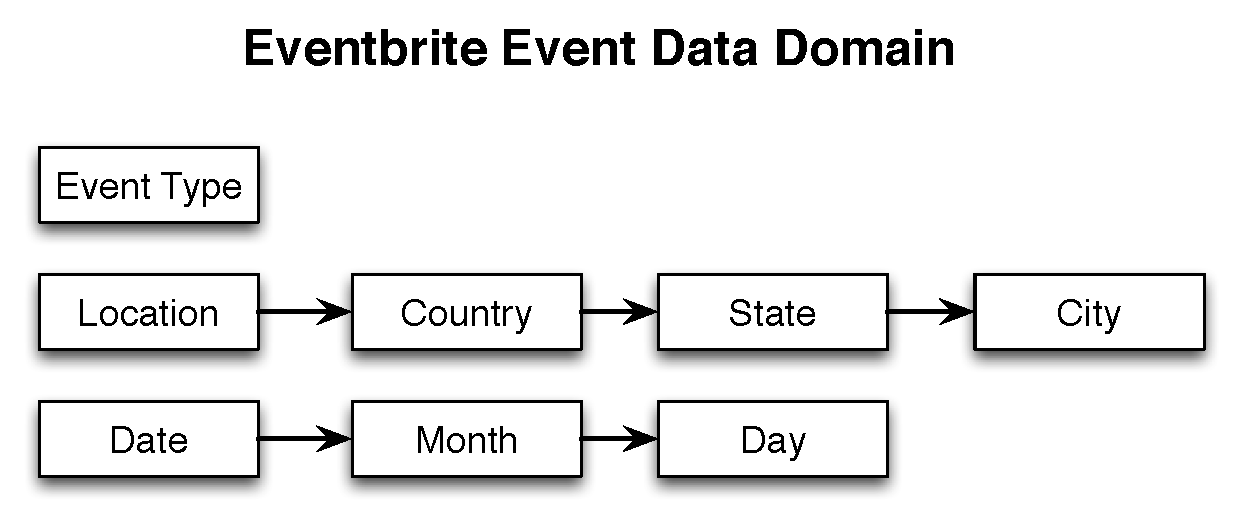
\includegraphics[clip,scale=0.4]{figs/eventsDomain.eps}
	\caption{The attributes describing the Eventbrite domain and the hierarchical structure of each attribute.}
	\label{fig:eventsdomain}
	\end{center}
	\vspace{-10pt}
\end{figure}

The domain $\domain$ can be viewed as a {\em lattice} corresponding to the crossproduct of all available hierarchies. Part of the lattice corresponding to the previous example is shown in \Cref{fig:eventslattice}. We denote this crossproduct as $\hierarchy$. We define a {\em point} in $\domain$ as a possible combination of values of {\em all} attributes. We will also refer to a collection of points for which only a subset of attributes shares the same value as a {\em slice} $\domain_P$ of $\domain$. For example, a slice of the event domain described above may correspond to concerts in Boston. The predicates describing this slice are EVENT TYPE = ``Concert", LOCATION = ``Boston, MA", DATE = ``*".  It is easy to see that each node in $\hierarchy$ represents a slice of the data domain $\domain$. 

\begin{figure}[h]
	\begin{center}
	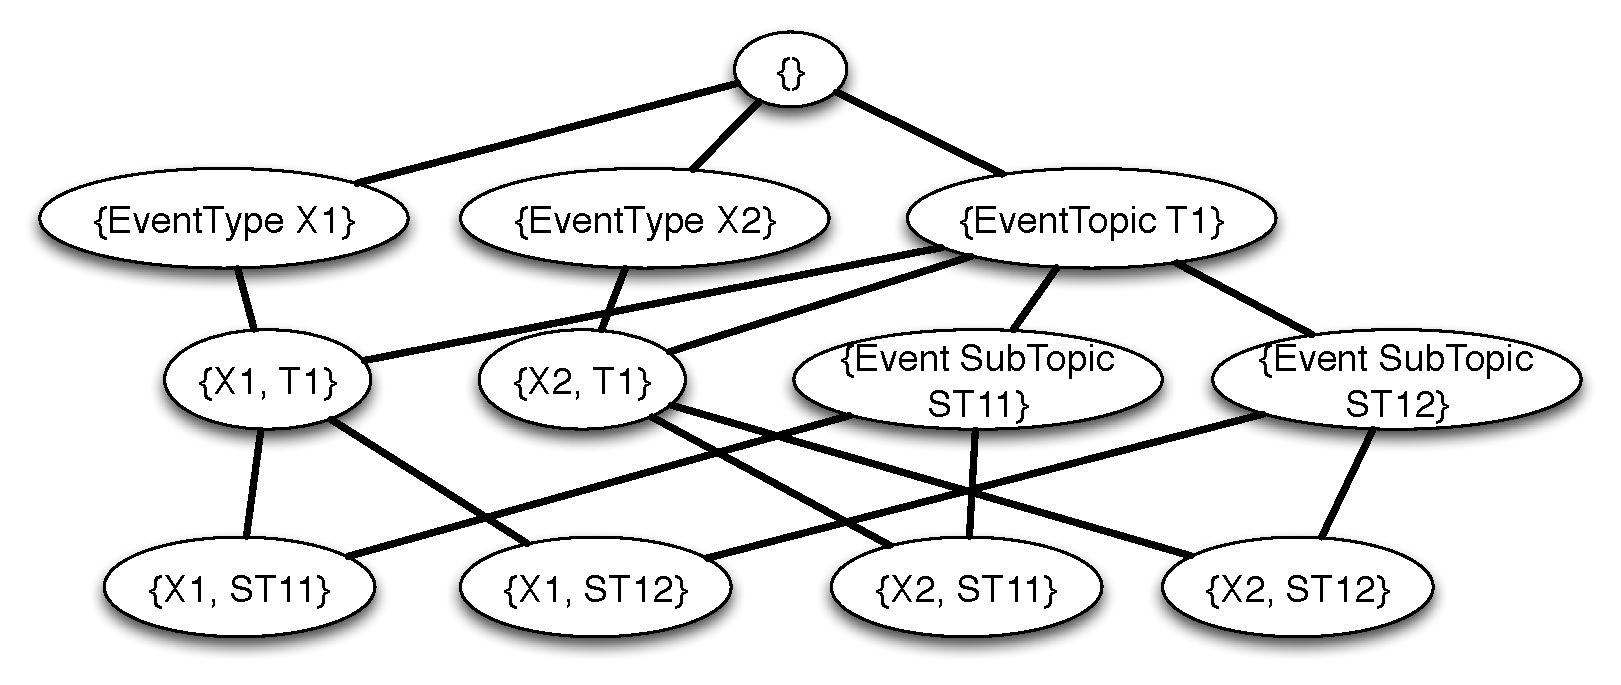
\includegraphics[clip,scale=0.32]{figs/eventsExLattice.eps}
	\caption{Part of the lattice defining the entire event entity domain described by the attributes in \Cref{fig:eventsdomain}.}
	\label{fig:eventslattice}
	\end{center}
	\vspace{-10pt}
\end{figure}

The basic version of {\em crowd entity extraction}~\cite{trushkowsky:2013} seeks to extract entities that belong in a {\em single} slice $\domain_P$ of $\domain$, specified by a set of predicates $P$ over a subset of attributes in $\attributes$. However, when considering large entity domains, such as the event domain, one may need to issue a series of entity extraction queries over multiple slices of $\domain$ - that may overlap with each other- so that the entire domain is covered. Issuing queries for different slices of the domain ensures that the coverage across the domain will be maximized. 

Let $\mathcal{P}(\domain)$ denote the set of all possible slices that their union covers the domain $\domain$. Moreover, let $\pi$ denote a {\em querying policy}, that is, a chain of crowd queries corresponding to different slices in $\mathcal{P}(\domain)$. Each query asks workers to provide entities corresponding to a slice $\domain_P$. Notice, that multiple queries can be issued against the same slice. Let $C(\pi)$ denote the overall cost, both in terms of monetary cost and latency, of a querying policy $\pi$. We define the gain of a querying policy $\pi$ as the total number of unique entities, denoted by $\uentities(\pi)$ extracted when following policy $\pi$. 

The above naturally gives raise to a tradeoff between the total number of extracted entities and the total cost. To optimize this tradeoff, previous work has proposed either a {\em pay-as-you-go} scheme~\cite{trushkowsky:2013} or a fixed answer size scheme~\cite{park:2014}. In the first case, one repeatedly issues queries to the crowd until the {\em marginal gain}, i.e., the difference between the new extracted entities and the querying cost, drops below a desired threshold. However, the proposed scheme does not enforce any budget constraints explicitly and focuses on a single query in isolation. Thus, it does not optimize the gain-cost tradeoff over an entire querying policy. In the second case, one repeatedly issues queries to the crowd until a desired number of entities is retrieved. The latter is specified by the user. Notice, that this assumes knowledge of the number of entities to be extracted, nevertheless, this information may not be available in many real-world scenarios. 

Here, we require that the user will {\em only} provide a monetary budget $\tau_c$ imposing a constraint on the total cost of a selected querying policy, and optimize over all possible querying policies across different slices of the data domain. Our goal is to identify the policy that maximizes the number of retrieved entities under the given budget constraint. More formally, we define the problem of budgeted crowd entity extraction as follows:

\begin{definition}[Budgeted Crowd Entity Extraction]
Let $\domain$ be a given entity domain and $\tau_c$ a monetary budget on the total cost of issued queries. The Budgeted Crowd Entity Extraction problem seeks to find 
a querying policy $\pi^*_S$ over a subset of slices $S \subseteq \mathcal{P}(\domain)$ that maximizes the number of unique entities extracted $\uentities(\pi^*_S)$ under the constraint $C(\pi^*_S) \leq \tau_c$.
\end{definition}

If $\domain$ is fully specified by a hierarchy $\hierarchy$ then $\mathcal{P}(\domain) = \hierarchy$. Thus, determining the optimal querying policy requires detecting the optimal subset of nodes in $\hierarchy$ to be queried so that the goal number of extracted entities is maximized under the given budget constraint. Notice that due to the different query configurations the optimal querying policy for the problem of budgeted crowd entity extraction should also identify the optimal configuration $(k,l)$ for each query in $\pi^*_S$.

The cost of a querying policy $\pi$ is defined as the total cost of all queries issued by following $\pi$. We have that $C(\pi) = \sum_{q \in \pi} c(q)$ where the cost of each query $q$ is defined according to a cost model specified by the user. Computing the total cost of a policy $\pi$ is easy. However, the gain $\uentities(\pi)$ of a policy $\pi$ is unknown as we do not know in advance the entities corresponding to each node in $\hierarchy$, and hence, needs to be estimated, as we discuss next. 

\subsection{Queries in Structured Domains}
\label{sec:sampling}
The entities in the domain are unknown. Moreover, we assume that the underlying entities exhibit different {\em popularity levels} with respect to crowd workers. These popularity levels can be formally defined using the notion of a probability distribution. In particular, the probability that an entity will appear in a query depends on its {\em popularity} in the overall entity population. The popularity of an entity is defined as the probability that this entity will appear in a query $q(1,0)$, i.e., a query asking for one entity from the population and using an exclude list of size zero. Since workers are asked to provide a limited number of entities as response to a query, each entity extraction query can be viewed as taking a random sample from an unknown population of entities. In the remainder of the paper, we will refer to the distribution characterizing the popularities of entities corresponding to a population as the {\em popularity distribution} of the population. 

Estimating the gain of a query $q(k,l)$ at a node $v \in \hierarchy$ is equivalent to estimating the number of new entities extracted by taking additional samples from the population of $v$ given all the retrieved entities by past samples associated with node $v$~\cite{trushkowsky:2013}. 

When extracting entities from a structured domain, the retrieved entities for a node $v$ can correspond to two different kinds of samples: (i) those that were extracted by considering the {\bf entire population} corresponding to node $v$ (ii) and those that we obtained by sampling {\bf only a part of the population} corresponding to $v$. Samples for a node $v$ can be obtained either by querying node $v$ or by indirect information flowing to $v$ by queries at other nodes in $\hierarchy$. We refer to the latter case as {\em dependencies across queries}. 
\begin{figure}[h]
	\begin{center}
	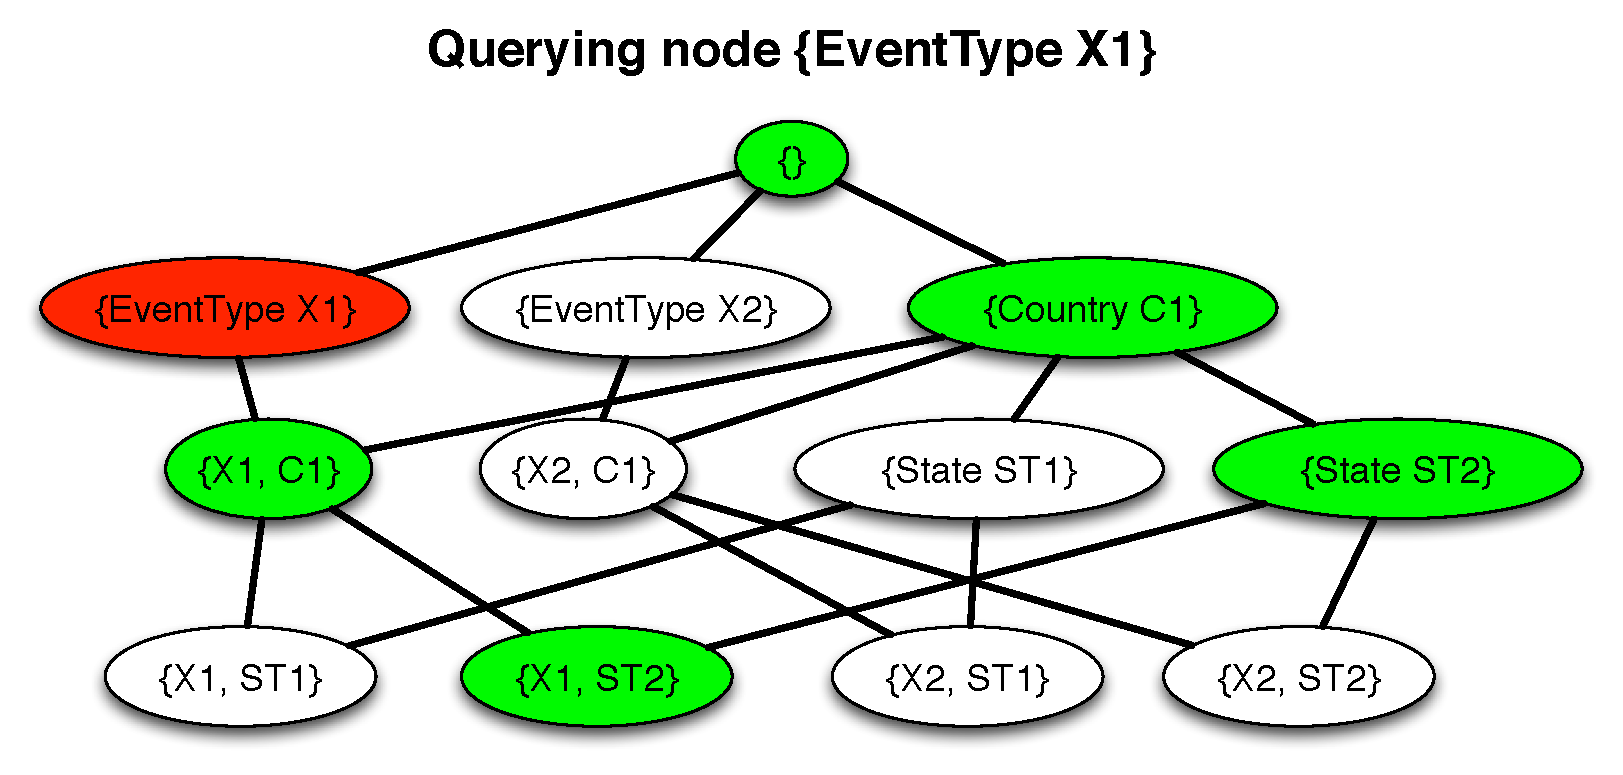
\includegraphics[clip,scale=0.32]{figs/exampleQuery.eps}
	\caption{An example query that extract an entity sample from the red node. The nodes marked with green correspond to the nodes for which indirect entity samples are retrieved.}
	\label{fig:query}
	\end{center}
	\vspace{-10pt}
\end{figure}

We use an example considering the lattice in \Cref{fig:eventslattice}, to illustrate these two cases. The example is shown in \Cref{fig:query}. Assume a query $q(k,0)$ issued against node \{EventType X1\}. Assume that the query result contains entities that correspond only to node \{X1,ST2\}. The green nodes in \Cref{fig:query} are nodes for which samples are obtained indirectly without querying them. Notice, that all these nodes, are ancestors of \{X1,ST2\}. Analyzing the samples for the different nodes we have:
\squishlist
\item The samples corresponding to nodes \{X1, C1\} and \{X1,ST2\} where obtained by considering their {\em entire population}. The reason is that node \{EventType X1\} is an ancestor of both and the entity population corresponding to it fully contains the populations of both \{X1,C1\} and \{X1,ST1\}. 
\item The samples corresponding to nodes \{ \}, \{Country C1\} and \{State ST2\} where obtained by considering only part of their population. The reason is that the population of node \{EventType X1\} does not fully contain the populations of these nodes. 
\squishend

Samples belonging to both types need to be considered when estimating the gain of a query at a node in $v \in \hierarchy$. To address this issue we merge the extracted entities for each node in $\hierarchy$ into a single sample and treat the unified sample as being extracted from the entire underlying population of the node. As we discuss later in \Cref{sec:solving} we develop querying strategies that traverse the lattice $\hierarchy$ in a top-down approach, hence, the number of samples belonging in the first category, i.e., samples retrieved considering the entire population of a node, dominates the number of samples retrieved by considering only part of a node's population. Moreover, it has been shown by Hortal et al.~\cite{hortal2006evaluating} that several of the techniques that can be used to estimate the gain of a query(see \Cref{sec:gain estimators}) present insensitivity to differences in the way the samples are aggregated.

%However, one cannot merge them directly into a single sample since samples that consider only part of the population for a node $v$ do not follow the same popularity distribution as samples that consider the entire population. To address, this challenge, we can view the process described above as an instance of {\em stratified sampling}. More precisely, given the hierarchical structure of the domain $\domain$, we can consider the population of each node in $\hierarchy$ as being split in multiple strata considering to the populations of its direct descendants. Following, this approach one can combine the aforementioned types of samples into a single stratified sample and use this observation to estimate the gain of different queries for the nodes in $\hierarchy$ (see \Cref{sec:gainestimators}).

\subsection{Framework Overview}
\label{sec:framework}
We present an overview of our proposed framework for solving the problem of budgeted crowd entity extraction over structured domains. We view the optimization problem described in \Cref{sec:extraction} as a multi-round adaptive optimization problem where at each round we solve the following subproblems: 
\squishlist 
\item \textbf{Estimating the Gain for a Query.} For each node in $v \in \hierarchy$, consider the retrieved entities associated with $v$ and estimate the number of new unique entities that will be retrieved if a new query $q(k,l)$ is issued at $v$. This needs to be repeat for all possible configurations of $k$ and $l$.
\item \textbf{Detecting the Optimal Querying Policy.} Using the gain estimates from the previous problem as input, identify the next (query, node) combination so that the total gain across all rounds is maximized with respect to the given budget constraint. 
\squishend
Our proposed framework iteratively solves the aforementioned problems until the entire budget is used. \Cref{fig:framework} shows a high-level diagram of our proposed framework. Throughout our framework, we assume that after issuing a query against the crowd, the retrieved answers can be associated with all relevant nodes across all attribute hierarchies, i.e., a worker will provide all the attribute values describing a reported entity. Dealing with incomplete information about entities is not the main focus of this paper and is part of the future work preposed in \Cref{sec:conclusions}.

\begin{figure}
	\begin{center}
	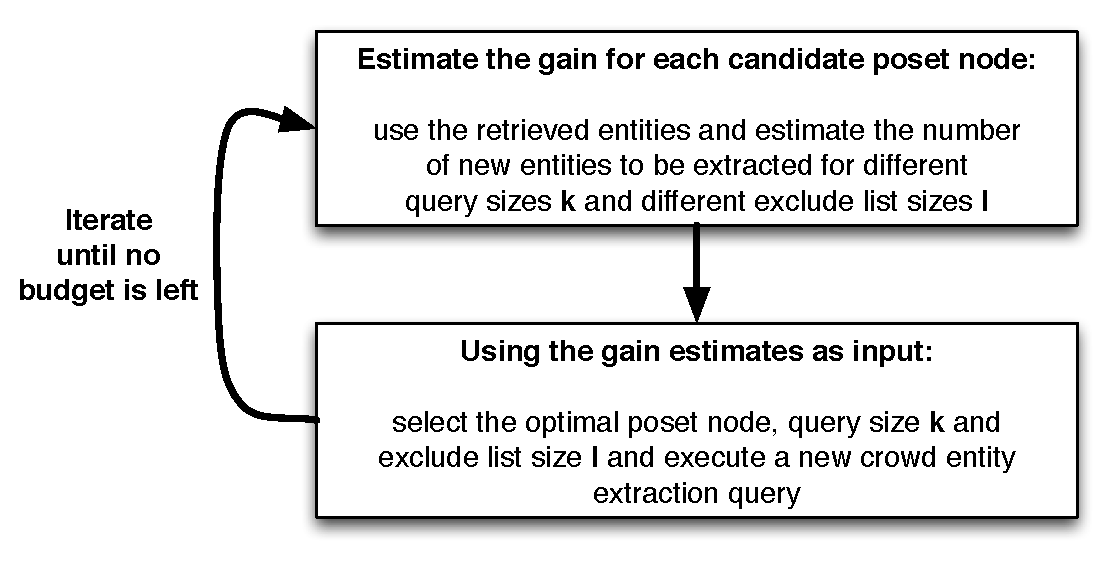
\includegraphics[clip,scale=0.45]{figs/framework.eps}
	\caption{Solution overview for budgeted entity extraction.}
	\label{fig:framework}
	\end{center}
	\vspace{-10pt}
\end{figure}

\section{Estimating the Gain of Queries}
\label{sec:gainestimators}
In this section, we present a novel lower bound for the return of a generalized query $q(k,l)$ at a node $v \in \hierarchy$. Previous work~\cite{trushkowsky:2013} has drawn connections between this problem and the literature of species estimation~\cite{chao:1992}. However,  the proposed techniques are agnostic to any structure exhibited by the domain under consideration and to the presence of an exclude-list-based query interface. In particular, the existing methodology does not proposed any techniques for estimating the number of new tuples extracted by a query when restricting the worker answer not to belong to a certain collection of entities. We first review the existing methodology for estimating the gain of a query, then we discuss how these estimators can be extended to consider an exclude list, and finally, we present a new methodology for estimating the gain of generalized queries $q(k,l)$. We first introduce our approach considering samples that are retrieved by the entire entity population corresponding to a node and then generalize it to stratified samples.

\subsection{Previous Estimators} 
Consider a specific node $v \in \hierarchy$. Prior work only considers samples retrieved from the entire population associated with $v$ and does not consider an exclude list. Let $Q$ be the set of all existing samples retrieved by issuing queries against $v$. These samples can be combined into a single sample of size $n = \sum_{q \in Q} {\sf size}(q)$. Let $f_i$ denote the number of entities that appear $i$ times in this unified sample, and let $f_0$ denote the number of unseen entities from the population under consideration. Finally, let $C$ be the population coverage of the unified sample.

A new query $q(k,0)$ at node $v$ can be viewed as increasing the size of the unified sample by $k$ elements. Prior work leveraged techniques from the species estimation literature to estimate the expected number of new entities returned in $q(k,0)$. Shen et al.~\cite{shen:2003}, derive an estimator for the number of new species $\hat{N}_{Shen}$ that would be found in an increased sample of size $k$. The approach assumes that the unobserved entities have equal relative popularity. An estimate of the unique elements found in an increased sample of size $k$ is given by:

\begin{equation}
\label{eq:shen}
\hat{N}_{Shen} = f_0\left( 1 - \left(1 - \frac{1 - C}{f_0}\right)^k\right)
\end{equation}

At a high-level, the second term of Shen's formula corresponds to the probability that at least one unseen entity will be present in a query asking for $k$ more entities. Thus, multiplying this quantity with the number of unseen entities $f_0$ corresponds to the expected number of unseen entities that will be present in the result of a new query $q(k,0)$.

Notice, that the quantities $f_0$ and $C$ are unknown and thus need to be estimated considering the entities in the running unified sample. The coverage can be estimated by considering the Good-Turing estimator $\hat{C} = 1 - \frac{f_1}{n}$ for the existing retrieved sample. On the other hand, multiple estimators have been proposed for estimating the number of unseen entities $f_0$. Trushkowsky et al.~\cite{trushkowsky:2013} proposed a variation of an estimator introduced by Chao et al.~\cite{chao:1992} to estimate $f_0$. Nevertheless, the authors argue that the original estimator proposed by Chao as well as their own estimator when estimating  the number of new unseen items in a query $q(k,0)$.

The estimator by Chao~\cite{chao:1992} on which the authors build has been shown to result in considerable negative bias in cases where the number of observed entities from a population represents only a small fraction of the entire population~\cite{hwang:2010}. To address this problem, Hwang and Shen~\cite{hwang:2010} proposed a regression based technique to estimate $f_0$. This estimator is shown to result in significantly smaller bias and empirically outperforms previously proposed estimators, including the one proposed by Chao, when the ratio of retrieved entities to the entire entity population is small. It also performs comparably to previous estimators when the ratio is larger. Notice, that the output of this estimator can also be used as a plug-in quantity in \Cref{eq:shen}. 
Thus in this paper we use the regression based estimator proposed by Hwang and Shen~\cite{hwang:2010} and in \Cref{sec:exps} we empirically show that it is better than the one proposed by Chao~\cite{chao:1992}.

However, both the aforementioned estimators are agnostic to an exclude list. Next, we discuss how one can estimate the return of a query $q(k,l)$ in the presence of an exclude list of size $l$.
\subsection{Queries With an Exclude List}
\label{sec:excludelist}
Consider an exclude list of size $l$. As discussed before an exclude list is a set of entities that correspond to invalid worker answers. Considering an exclude list for a query at a node $v \in \hierarchy$ corresponds to limiting our sampling to a restricted subset of the entity population corresponding to node $v$. In fact, we want to estimate the expected return of a query of size $k$ conditioning on the fact that the entities in the exclude list will not be retrieved by any new sample. The latter corresponds to removing these entities from the population under consideration. Thus, the estimates $\hat{f}_0$ and $\hat{C}$ should be updated before applying \Cref{eq:shen} to compute the expected return of a query of size $k$. This can be done by removing the entities included in the exclude list from the running sample for node $v$, recomputing the entity counts $f_i$ and following the techniques presented above for computing the updated estimates for $\hat{f}_0$ and $\hat{C}$. This approach requires that the exclude list is known in advance. To construct an exclude list on can follow a randomized approach, where $l$ of the retrieved entities are including in the list uniformly at random. 

\subsection{Regression Based Gain Estimation}
\label{sec:newestim}
Building upon the approach of Hwang and Shen~\cite{hwang:2010}, we introduce a new technique for estimating the gain of a generalized query $q(k,l)$ directly without using the estimator shown in \Cref{eq:shen}. Since we want to estimate the gain even for nodes with a small number of retrieved entities we propose a regression based technique that is able to capture the structural properties of the expected gain function as discussed below. 

To derive the new lower bound we make used of the generalized jackknife procedure for species richness estimation. Given two (biased) estimators of $S$, say $\hat{S}_1$ and $\hat{S}_2$, let $R$ be the ratio of their biases:
\begin{equation}
R = \frac{E(\hat{S}_1) - S}{E(\hat{S}_2) - S}
\end{equation}
By the generalized jackknife procedure, we can completely eliminate the bias resulting from either $\hat{S}_1$ or $\hat{S}_2$ via
\begin{equation}
S = G(\hat{S}_1, \hat{S}_2) = \frac{\hat{S}_1 - R\hat{S}_2}{1 - R}
\label{eq:jknife}
\end{equation}
provided the ratio of biases $R$ is known. However, $R$ is unknown and we need to estimate it. 

Let $D_n$ denote the number of unique entities in a unified sample of size $n$. We consider the following two biased estimators of $S$: $\hat{S_1} = D_n$ and $\hat{S}_2 = \sum_{j=1}^n D_{n-1}(j)/n = D_n - f_1/n$ where $D_{n-1}(j)$ is the number of species discovered with the $j$th observation removed from the original sample. Replacing these estimators in \Cref{eq:jknife} gives us:
\begin{equation}
S = D_n +\frac{R}{1-R}\frac{f_1}{n}
\end{equation}

Similarly, for a sample of increased size $n+m$ we have:
\begin{equation}
S = D_{n+m} +\frac{R^{\prime}}{1-R^{\prime}}\frac{f^{\prime}_1}{n+m}
\end{equation}
where $R^{\prime}$ is the ratio of the biases and $f^{\prime}_1$ the number of singleton entities for the increased sample.

Let $K = \frac{R}{1-R}$ and $K^{\prime} = \frac{R^{\prime}}{1-R^{\prime}}$. Taking the difference of the previous two equations we have:
\begin{equation}
D_{n+m} - D_{n} = K\frac{f_1}{n} - K^{\prime}\frac{f^{\prime}_1}{n+m}
\end{equation}

Therefore, we have:
\begin{equation}
\label{eq:new}
new = K\frac{f_1}{n} - K^{\prime}\frac{f^{\prime}_1}{n+m}
\end{equation}

We need to estimate $K$, $K^{\prime}$ and $f^{\prime}_1$. We start with $f^{\prime}_1$ denoting the number of singleton in the increased sample of size $n+m$. Notice, that $f^{\prime}_1$ is not known since we have not obtained the increased sample yet, so we need to express it in terms of $f_1$, i.e., the number of singletons, in the running sample of size $n$. We have:
\begin{equation}
f^{\prime}_1 = new + f_1 - f_1*\Pr[\mbox{in query of size m}]
\end{equation}
Following an approach similar to Shen et al.~\cite{shen:2003}, we have that the probability of a singleton appearing in a query of size $m$ is:
\begin{equation}
\Pr[\mbox{in query of size m}] = \sum_{k=0}^m(1-(1-\frac{1}{f_1})^k) {m \choose k}(1-p_1)^k p_1^{m-k}
\end{equation}
where $p_1$ denotes the probability that a singleton item in the sample of size $n$ will be selected in a future query. We estimate this probability using the corresponding Good-Turing estimator considering the running sample. We have:
\begin{equation}
p_1 = \hat{\theta}(1) = \frac{1}{n}2\frac{N_2}{N_1}
\end{equation} 
where $N_2$ is the number of entities that appear twice in the sample and $N_1$ is the number of singletons. 
Eventually we have that:
\begin{align}
f^{\prime}_1 &= new + f_1(1- \sum_{k=0}^m(1-(1-\frac{1}{f_1})^k) {m \choose k}(1-p_1)^k p_1^{m-k}) \nonumber \\
f^{\prime}_1 &= new + f_1(1- P)
\end{align}
Replacing the last equation in \Cref{eq:new} we have:
\begin{align}
&new = K\frac{f_1}{n} - K^{\prime}\frac{new + f_1(1- P)}{n+m} \nonumber \\
&new = K\frac{f_1}{n} - K^{\prime}\frac{new}{n+m} - K^{\prime}\frac{f_1(1- P)}{n+m} \nonumber \\
&new(1 + \frac{K^{\prime}}{n+m}) = K\frac{f_1}{n} - K^{\prime}\frac{f_1(1- P)}{n+m} \nonumber \\
&new = \frac{1}{(1 + \frac{K^{\prime}}{n+m})}(K\frac{f_1}{n} - K^{\prime}\frac{f_1(1- P)}{n+m}) \nonumber
\end{align}

Next, we discuss how one can estimate $K$ and $K_{\prime}$. To estimate $K$ we follow the regression approach introduced by Hwang and Shen~\cite{hwang:2010}. From the Cauchy-Schwarz inequality we have that:
\begin{equation}
K = \frac{\sum_{i=1}^S (1-p_i)^n}{\sum_{i=1}^S p_i(1-p_i)^{n-1}} \geq \frac{(n-1)f_1}{2f_2}
\end{equation}
This can be generalized to:
\begin{equation}
K=\frac{nf_0}{f_1} \geq \frac{(n-1)f_1}{2f_2} \geq \frac{(n-2)f_2}{3f_3} \geq \dots
\end{equation}
Let $g(i) = \frac{(n-i)f_i}{(i+1)f_{i+1}}$. From the above we have that the function $g(x)$ is a smooth monotone function for all $x \geq 0$. Moreover, let $y_i$ denote a realization of $g(i)$ mixed with a random error. Hwang and Shen how one can use an exponential regression model to estimate $K$. The proposed model corresponds to:
\begin{equation}
y_i = \beta_0\exp(\beta_1i^{\beta_2}) + \epsilon_i
\end{equation}
where $i = 1, \dots, n-1$, $\beta_0 > 0$, $\beta_1 < 0$, $\beta_2 >0$ and $\epsilon_i$ denotes random errors. It follows that $K = \beta_0$. 

Finally, we show how one can estimate the value of $K_\prime$ for an increased sample of size $n+m$. First, we show that $K$ increases monotonically as the size of the running sample increases. Let $K(n) = \frac{\sum_{i=1}^S (1-p_i)^n}{\sum_{i=1}^S p_i(1-p_i)^{n-1}}$ be a function returning the value of $K$ for a sample of size $n$. We have the following lemma. 

\begin{lemma}
We have $K(n+m) \geq K(n), \forall n,m > 0$.
\end{lemma}
\begin{proof}
In the remainder of the proof we will denote $K(n+m)$ as $K^{\prime}$. By definition we have that $K = \frac{\sum_{i=1}^S (1-p_i)^n}{\sum_{i=1}^S p_i(1-p_i)^{n-1}}$ and $K^{\prime} = \frac{\sum_{i=1}^S (1-p_i)^{n+m}}{\sum_{i=1}^S p_i(1-p_i)^{n+m-1}}$. We want to show that:
{\small
\begin{align}
&\frac{\sum_{i=1}^S (1-p_i)^{n+m}}{\sum_{i=1}^S p_i(1-p_i)^{n+m-1}} \geq \frac{\sum_{i=1}^S (1-p_i)^n}{\sum_{i=1}^S p_i(1-p_i)^{n-1}} \nonumber \\
&\sum_{i=1}^S (1-p_i)^{n+m}\sum_{j=1}^S p_j(1-p_j)^{n-1} \geq \sum_{i=1}^S p_i(1-p_i)^{n+m-1}\sum_{j=1}^S (1-p_j)^n\nonumber \\
&\sum_{i,j:i\prec j}[(1-p_i)^{n+m}p_j(1-p_j)^{n-1} - p_i(1-p_i)^{n+m-1}(1-p_j)^n + \nonumber \\
& + (1-p_j)^{n+m}p_i(1-p_i)^{n-1} - p_j(1-p_j)^{n+m-1}(1-p_i)^n] \geq 0 \nonumber \\
&\sum_{i,j:i\prec j}[(1-p_i)^{n}(1-p_j)^{n-1}p_j((1-p_i)^{m} - (1-p_j)^{m})  + \nonumber \\
& - (1-p_j)^{n}p_i(1-p_i)^{n-1}((1-p_i)^{m} - (1-p_j)^{m}) \geq 0 \nonumber \\
&\sum_{i,j:i\prec j}[(1-p_i)^{n-1}(1-p_j)^{n-1}(p_j-p_i)((1-p_i)^{m} - (1-p_j)^{m}) \geq 0
\end{align}}

But the last inequality always holds since each term of the summation is positive. In particular, if $p_j \geq p_i$ then
also $1-p_i \geq 1-p_j$ and if $p_j \leq p_i$ then $1-p_i \leq 1-p_j$.
\end{proof}

We have that $K(n)$ is an increasing function of the sample size. Moreover, $K(n)$ has a decreasing slope. We model $K$ as a generalized logistic function of the form $f(x) = \frac{A}{1+exp(-G(x-D))}$. As we observe samples of different sizes for different queries we estimate $K$ as described above and therefore we observe different realizations of $f(\cdot)$. Thus, we can learn the parameters of $f$ and use it to estimate $K^{\prime}$. In the presence of an exclude list of size $l$ we follow the approach described in \Cref{sec:excludelist} to update the quantities $f_i$ used in the analysis above. 

\subsection{Negative Answers and Gain Estimation}
Next, we study the effect of {\em negative answers} on estimating the gain of future queries. It is possible to issue a query at a specific node $v \in \hierarchy$ and receive no entities, i.e., we receive a negative answer. This is an indication that the underlying entity population of $v$ is empty. In such scenarios we assign the expected gain of future queries at $v$ and all its descendants to zero. 

Another type of negative answer corresponds to the scenario where we issue a query at an ancestor node $u$ of $v$ and receive no entities associated with $v$ but received some entities for $u$. Notice, that in this case we do not have enough information to update our estimates for node $u$. The reason is that due to the restricted query size entities from other descendants of $u$ may be more popular with respect to the popularity distribution of $u$.

%\subsection{Estimation with Stratified Samples}
%The previous estimators can only be used when the samples for a node $v \in \hierarchy$ have been retrieved considering its entire entity population. However, as discussed in \Cref{sec:sampling} this is not always the case in hierarchically structured domains as we may have stratified samples for the nodes in $\hierarchy$. In this case one needs to take into account how the entities in the result of a query $q(k,l)$ at node $v$ are distributed across its direct descendants, i.e., the strata corresponding to $v$. Let $k$ be the total number of entities in the query result and $C(v)$ the set of direct descendants of $v$. According to propionate stratification we have that $k = \sum_{c \in C(v)} \frac{n_c}{\sum_c \in C(v) n_c} k$ where $n_c$ denotes the number of entities in descendant $c$ obtained only by querying node $v$ directly. Notice, that the quantity $\frac{n_c}{\sum_c \in C(v) n_c}$ corresponds to the probability that an entity in the query result will be retrieved by the population corresponding to descendant $c$.  To account for descendants for which no entities have been retrieved, we consider a smoothed version of the previous equation, i.e., $k = \sum_{c \in C(v)} \frac{n_c + 1}{\sum_c \in C(v) n_c+ 1} k$. 
%
%Let $r(q(k,l),v)$ denote the gain by issuing query $q(k,l)$ at node $v \in \hierarchy$. The exclude list of size $l$ for node $v$ can be constructed by considering all the entities associated with $v$, and can be partitioned accordingly across the direct descendants of $v$ resulting to $|C(v)|$ exclude lists of size $l_c$ for each descendant node $c \in C(v)$.  Combining this with the proportionate stratification of the query result, we can estimate $r(q(k,l),v)$ as:
%\begin{equation}
%r(q(k,l),v) = \sum_{c \in C(v)} r(q(\frac{n_c + 1}{\sum_c \in C(v) n_c+ 1} k,l_c),c)
%\end{equation}
%
%If the entities in a descendant node $c \in C(v)$ have been retrieved only by considering the entire population corresponding to $c$, one can use the approach presented in \Cref{sec:newestim} to estimate the quantity $r(q(\frac{n_c + 1}{\sum_c \in C(v) n_c+ 1} k,l_c),c)$. Otherwise, one needs to recursively apply the technique proposed here. 
%
%\noindent \textbf{Discussion.} Applying the approach of proportionate stratification can be prohibitively expensive due to the exponential size of lattice $\hierarchy$. Therefore, one can estimate $r(q(k,l),v)$ by computing the quantities $r(q(\frac{n_c + 1}{\sum_c \in C(v) n_c+ 1} k,l_c),c), \forall c \in C(v)$ using the estimator proposed in \Cref{sec:newestim}. While, the latter ignores the presence of stratified samples can significantly speed up the corresponding computations. 

\section{Discovering Querying Policies}
\label{sec:solving}
In this section, we focus on the second component of our proposed algorithmic framework. In particular, we introduce a multi-round adaptive optimization algorithm for identifying a querying strategy that will maximize the total gain across all rounds under the given budget constraints. The algorithmic framework we propose builds upon ideas from the multi-armed bandit literature~\cite{Auer:2003,EvenDar06actionelimination}. In particular,  at each round the proposed algorithm uses as input the estimated return for queries $q(k,l)$ at the different nodes in $\hierarchy$. Before presenting our proposed algorithm we list several challenges associated with this adaptive optimization problem.

\begin{enumerate}
\item The first challenge is that the number of nodes in $\hierarchy$ is exponential with respect to the number of attributes $\attributes$ describing the domain of interest. Querying every possible node to estimate its expected return for different queries $q(k,l)$ is prohibitively expensive. In fact, it is natural to assume a budget that does not allow any algorithm to query all nodes in the hierarchy. However, we assume that keeping estimates for each of the nodes for which at least one entity has been retrieved is feasible. 
\item The second challenge is balancing there tradeoff between {\em exploitation} and {\em exploration}~\cite{Auer:2003}. The first refers to querying nodes for which sufficient entities have been retrieved and hence we have an accurate estimate for their expected return while the latter refers to exploring new nodes in $\hierarchy$ in order to avoid locally optimal policies.
\end{enumerate}

\subsection{Balancing Exploration and Exploitation}
While issuing different queries $q(k,l)$ at different nodes of $\hierarchy$ we obtain a collection of entities that can be assigned to different nodes in $\hierarchy$. For each such node we can estimate the return of a new query $q(k,l)$ using the estimator presented in \Cref{sec:newestim}. However, this estimate is based on a rather small sample of the underlying population. Thus, exploiting this information at every round may need to suboptimal decision. This is the reason why one needs to balance the trade-off between exploiting nodes for which the estimated return is high and nodes that haven't been queried many times. Formally, the latter corresponds to upper bounding the expected return of each potential action with a confidence interval that depends on both the variance of the expected return and the number of times an action is evaluated.

Let $r(\alpha)$ denote the expected return of action $\alpha$ that is an estimate of the true return $r^*(\alpha)$. Moreover, let $\mathcal{E}(\alpha)$ be an error component on the return of action $\alpha$ chosen such that $r(\alpha) - \sigma(\alpha) \leq r^*(\alpha) \leq r(\alpha) + \sigma(\alpha)$ with high probability. The parameter $\sigma(\alpha)$ should take into account both the empirical variance of the expected return as well as our uncertainty if an action has been chosen few times. Let $n_{\alpha,t}$ be the number of times we have chosen action $\alpha$ by round $t$, and let $v_{\alpha,t}$ denote the maximum between some constant $c$ (e.g., $c = 0.01$) and the empirical variance for action $\alpha$ at round $t$. The latter can be computed using bootstrapping over the estimator presented in \Cref{sec:newestim}. Several techniques have been proposed in the multi-armed bandits literature to compute the parameter $\sigma(\alpha)$~\cite{teytaud:inria-00173263}. Teytaud et al.~\cite{teytaud:inria-00173263} showed that techniques considering both the variance and the number of times an action has been chosen tend to outperform other proposed methods. Based on this observation, we choose to use the following formula for sigma:
\begin{equation}
\sigma(\alpha) = \sqrt{\frac{v_{\alpha,t}\cdot\log(t)}{n_{\alpha,t}}}
\end{equation}

\subsection{A Heuristic for Querying Policies}
We now introduce our proposed multi-round algorithm for solving the budgeted entity enumeration problem. At a high-level our algorithm proceeds as follows: Let $\mathcal{S}$ denote the set of all potential queries $q(k,l)$ that can be issued at the different nodes of $\hierarchy$ during a round $r$. Moreover, let $f(\alpha)$ and $c(\alpha)$ denote the upper bounded return (i.e., gain) and cost for an action $\alpha \in \mathcal{S}$. At round $r$ the algorithm identifies an action in $\mathcal{S}$ that maximizes the quantity $\frac{f(\alpha)}{c(\alpha)}$ under the constraint that the cost of action $\alpha$ is less or equal to the remaining budget. Since we are operating under a specified budget one can view the problem in hand as a variation of the typical knapsack problem. If no such action exists then the algorithm terminates. Otherwise the algorithm issues the query corresponding to action $\alpha$, updates the set of unique entities obtained from the queries, the remaining budget and updates the set of potential queries $q(k,l)$ that can be executed in the next round.  An overview of the proposed algorithm is shown in Algorithm \ref{algo:overall}. 

As discussed before, the size of $\hierarchy$ is exponential to the values of attributes describing it, and thus, considering all the possible queries corresponding to the different nodes of the hierarchy can be prohibitively expensive. Next, we discuss how one can initialize and update the set of potential actions as the algorithm progresses considering the structure of the lattice $\hierarchy$ and the retrieved entities from previous rounds. 

\begin{algorithm}[h]
\caption{Overall Algorithm}
\label{algo:overall}
\begin{algorithmic}[1]
\STATE {\bf Input:} $\hierarchy$: the hierarchy describing the entity domain; $f$: value oracle access to gain upper bound; $c$: value oracle access to the query costs; $\beta_c$: query budget;
\STATE {\bf Output:} $\uentities$: a set of extracted distinct entities;
\STATE $\uentities \leftarrow \{\}$
\STATE $RB \leftarrow \beta_c$ /* Initialize remaining budget */
\STATE $\mathcal{S} \leftarrow$ {\sf UpdateActionSet($\hierarchy$)}
\WHILE {$RB > 0$ and $S \neq \{\}$}
	\STATE $\alpha \leftarrow \arg\max_{\alpha \in {\mathcal{S}}} \frac{f(a)}{c(a)}$ such that $RB - c(a) >0$
	\IF {$\alpha$ is NULL }
		\STATE break;
	\ENDIF
	\STATE $RB \leftarrow RB - c(a)$ /* Update budget */
	\STATE Issue query corresponding to $\alpha$
	\STATE $E \leftarrow$ entities from query
	\STATE $\uentities \leftarrow \uentities \cup E$ /* Update unique entities */
	\STATE $\mathcal{S} \leftarrow$ {\sf UpdateActionSet($\hierarchy$)}
\ENDWHILE
\RETURN $\uentities$
\end{algorithmic}
\end{algorithm}

\subsection{Updating the Set of Actions}
Due to the exponential size of the lattice $\hierarchy$ we need to limit the set of possible actions Algorithm~\ref{algo:overall} considers. To avoid keeping estimates for actions with bad returns we exploit the structure the given domain $\hierarchy$. We propose an algorithm that updates the set of actions by traversing the input lattice in a bottom-down manner extending it by adding new actions that corresponds to queries for nodes that are {\em direct descendants} of already queried nodes.

The intuition behind this approach is the following. It is easy to see that due to the hierarchical structure of the lattice nodes at higher levels of the lattice corresponds to larger populations of entities. Therefore, issuing queries at these nodes can potentially result to a larger number of extracted entities. Also, traversing the lattice in a bottom-down fashion allows one to detect sparsely populated areas of the lattice and hence avoid spending any of the available budget on issuing queries corresponding to them.

In more detail, our approach for updating the set of available actions (Algorithm~\ref{algo:updateactions}) proceeds as follows: If the set of available actions is empty start by considering all possible queries that can be issued at the root of $\hierarchy$ (Ln. 4-5). The set of possible queries corresponds to queries $q(k,l)$ for all combinations of the values of parameters $k$ and $l$. Recall that these are pre-specified by the designed of the querying interface. If the set of available actions is not empty, we consider the node associated with the action selected in the last round and populate the set of available actions with all the queries corresponding to its direct descendants (Ln. 7-9). As mentioned above the number of nodes in $\hierarchy$ can be prohibitively large, therefore we also remove any {\em bad actions} from the running set of actions (Ln.  10-14). 
An action $\alpha$ is bad when $r(\alpha) + \sigma(\alpha) < \max_{\alpha^{\prime} \in \mathcal{S}} (r(\alpha^{\prime}) - \sigma(\alpha^{\prime}))$. Intuitively, this inequality states that we do not need to consider again an action as long as there exists another action such that the upper bounded return of the former is lower than the lower bounded return of the latter. This is a standard technique adopted in multi-armed bandits to limit the number of actions considered by the algorithm~\cite{EvenDar06actionelimination}. 
\begin{algorithm}[h]
\caption{UpdateActionSet}
\label{algo:updateactions}
\begin{algorithmic}[1]
\STATE {\bf Input:} $\hierarchy$: the hierarchy describing the entity domain; $u$: a node in $\hierarchy$ associated with the last selected action; $\mathcal{S}_{old}$: the running set of actions; $V_k$: set of values for query parameter $k$; $V_l$: set of values for query parameter $l$;
\STATE {\bf Output:} $\mathcal{S}_{new}$: the updated set of actions;
\STATE \textbf{/* Extend Set of Actions*/}
\IF {$\mathcal{S}_{old}$ is empty}
	\RETURN $\{$Root of $\hierarchy \}$
\ENDIF 
\STATE $\mathcal{S}_{new} \leftarrow \mathcal{S}_{old}$
\FORALL{$d \in ${\sf Set of Direct Descendant Nodes of $u$}}
\STATE $A_d \leftarrow$ Set of queries at $u$ for all configurations in $V_k \times V_l$
\STATE $\mathcal{S}_{new} \leftarrow \mathcal{S}_{new} \cup A_d$
\ENDFOR
\STATE \textbf{/* Remove Bad Actions*/}
\STATE /* Find maximum lower bound on gain over all actions in $\mathcal{S}_{new}$*/
\STATE $thres \leftarrow \max_{\alpha^{\prime} \in \mathcal{S}_{new}} (r(\alpha^{\prime}) - \sigma(\alpha^{\prime}))$  
\STATE $\mathcal{B} \leftarrow$ All actions $a$ in $\mathcal{S}_{new}$ with $r(\alpha) + \sigma(\alpha) < thres$
\STATE $\mathcal{S}_{new} \leftarrow \mathcal{S}_{new} \setminus \mathcal{B}$
\RETURN $\mathcal{S}_{new}$
\end{algorithmic}
\end{algorithm}

\section{Experimental Evaluaiton}
\label{sec:exps}
In this section we present an empirical evaluation of our proposed algorithmic framework.

\section{Related Work}
\label{sec:related}

\ \\Beth's work
\ \\Work by Yael Amsterdamer on Crowd Mining
\ \\CrowdFill work by Stanford

\section{Conclusions}
\label{sec:conclusions}


\bibliographystyle{abbrv}
\bibliography{crowd_hierarchies}

\end{document}
